\section{Hardware algorithm accelerator (uDSC)\label{sec:hardware-accelerator}}

\subsection{uDSC Overview}

\bilingal{%
数字运算加速器(uDSC)作为 LGT8XM 内核的一个运算协处理模块,配合 LGT8XM 内核
16 位 LD/ST 模式,实现一个 16 位的数字信号处理单元。可以满足大部分控制类数字信号的处理。
uDSC 功能内部以及功能:
\begin{itemize}
\item 16 位操作数寄存器 DX/DY
\item 32 位累加寄存器 DA3. 单周期 17 位乘法器(可以实现 16 位有/无符号乘法运算)
\item 单周期 17 位乘法器(可以实现 16 位有/无符号乘法运算)
\item 32 位 ALU (可以实现 16/32 位的加法,减法以及移位运算)
\item 16 位饱和运算 (用于将运算结果存储到 RAM 空间)
\item 32/16 除法器,8 个周期内完成运算
\end{itemize}
}{%
Digital Arithmetic Accelerator (uDSC), an co-processor arithmetic module of
LGT8XM, in combined with 16 bit LD/ST mode, features as a 16 bit digital pulse
processing unit. It can deal with most control digital pulse. uDSC internal
function as below:
\begin{itemize}
\item 16 bit operand register DX/DY
\item 32 BIT accumulator register DA
\item Single circle 17 bit multiplier (feature 16 bit multiply algorithm with/without symbol)
\item 32-bit ALU (feature 16/32 bit plus, minus and shift operation)
\item 16-bit saturation arithmetic ( to save algorithm result to RAM memory)
\item 32/16 divider, algorithm within 8 cycles
\end{itemize}
}

\begin{figure}[tb]
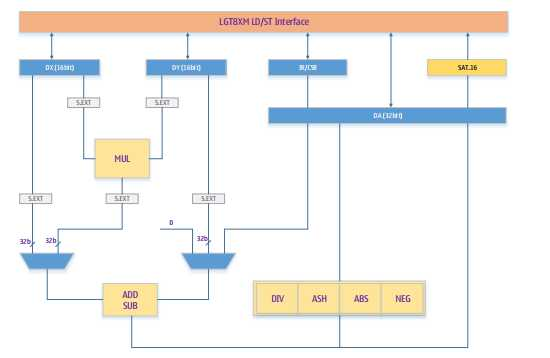
\includegraphics[width=\columnwidth]{Images/f-028}
\caption{uDSC high-level architecture.}
\end{figure}


\subsection{Register definition}
\begin{tabular}{ccl}
\toprule
Name & IO Address & Comments\\
\midrule
DCSR & 0x20(0x00) & uDSC control status register \\
DSIR & 0x21(0x01) & Arithmetic instruction register \\
DSSD & 0x22(0x02) & Result of 16-bit saturation arithmetic of accumulator DSA \\
DSDX & 0x10(0x30) & Operands DSDX, 16-bit read and write access \\
DSDY & 0x11(0x31) & Operands DSDY, 16-bit read and write access \\
DSAL & 0x38(0x58) & 32-bit accumulator DSA[15:0], 16-bit read and write access \\
DSAH & 0x39(0x59) & 32-bit accumulator DSA[31:16], 16-bit read and write access \\
\bottomrule
\end{tabular}

\subsection{DSCR: Control Status Register}

\begin{description}
\item[Address] \texttt{0x20 (0x00)}
\item[Default value] \texttt{0010\_xxxx}
\end{description}

\begin{tabular}{ccccccccc}
\toprule
Bit & 7 & 6 & 5 & 4 & 3 & 2 & 1 & 0 \\
\midrule
Name & DSUEN & MM & D1 & D0 & -- & N & Z & C \\
R/W & R/W & R/W & R/W & R/W & -- & R/W & R/W & R/W \\
\bottomrule
\end{tabular}

\begin{description}
\item[7  DSUEN]    uDSC module enable control: 1= enable,; 0=disable

\item[6  MM   ]    uDSC register mapping mode, for details referring to
introduction on 16-bit working mode 0=quick access mode; 1= IO mapping mode

\item[5  D1   ]    Division arithmetic, 1= done
\item[4  D0   ]    \bilingal{除法运算除 0 标志位}{Division arithmetic by zero flag}
\item[3  --   ]    Unimplemented
\item[2  N    ]    Arithmetic result is minus flag
\item[1  Z    ]    Arithmetic result is zero flag
\item[0  C    ]    \bilingal{32 加法器进位/借位标志}{32 Adder carry/borrow}
\end{description}

\subsection{uDSC case study}

\bilingal{%
下面为一个简单子程序(AVRGCC),实现一个 16 位的乘法运算,返回 32 位结果.:
}{%
Below is a very simple subroutine (AVRGCC), featuring a 16-bit multiply
arithmetic while return a 32-bit result:%
}

\lstinputlisting[language={[x86masm]Assembler}]{Listings/udsc.S}